\documentclass[11pt]{article}

\usepackage[a4paper,margin=1in]{geometry}
\usepackage[T1]{fontenc}
\usepackage[utf8]{inputenc}
\usepackage{lmodern}
\usepackage{microtype}
\usepackage{graphicx}
\usepackage{xcolor}
\usepackage{hyperref}
\usepackage{enumitem}
\usepackage{array}
\usepackage{booktabs}
\usepackage{fancyvrb}
\usepackage{titlesec}

\graphicspath{{../}}

\definecolor{ink}{HTML}{111111}
\definecolor{muted}{HTML}{666666}
\definecolor{gold}{HTML}{F2D36B}
\definecolor{softgold}{HTML}{FFF3C8}
\definecolor{line}{HTML}{E6E6E6}

\hypersetup{
  colorlinks=true,
  linkcolor=ink,
  urlcolor=ink,
  pdftitle={TaxBench-AU: A benchmark for testing whether AI agents can calculate Australian tax},
  pdfauthor={}
}

\titleformat{\section}{\Large\bfseries\color{ink}}{}{0pt}{}
\titlespacing*{\section}{0pt}{2.0em}{0.7em}

\setlength{\parindent}{0pt}
\setlength{\parskip}{0.8em}
\setlist[itemize]{leftmargin=1.4em,itemsep=0.25em,topsep=0.25em}

\newcommand{\captiontext}[1]{%
  {\small\color{muted}#1}%
}

\newenvironment{questionbox}
  {\par\medskip\noindent\begin{center}\begin{minipage}{0.92\linewidth}\setlength{\parskip}{0.55em}\hrule\vspace{0.9em}}
  {\vspace{0.2em}\hrule\end{minipage}\end{center}\medskip}

\begin{document}

{\small\color{muted}May 2026 -- Dataset report}

\vspace{0.8em}

{\LARGE\bfseries TaxBench-AU: A benchmark for testing whether AI agents can calculate Australian tax\par}

\section{Why this benchmark exists}

Australian tax is a hard test for AI agents.

The law is detailed, the rules change over time, and small facts can change the answer. Even experienced practitioners do not rely on memory alone. They check the legislation, the ATO guidance, the income year, the thresholds, and the exact wording of the scenario.

That makes tax a useful place to test AI. A tax agent that drafts advice, answers client questions, or helps with compliance can save time. But a confident wrong answer can also create real risk. To trust these systems, we need to know more than whether they sound fluent. We need to know whether they can read the facts, apply the right rule, do the calculation, and choose the correct result.

Generic AI benchmarks do not measure that. A high score on a broad benchmark does not tell us whether a model can apply the CGT discount, calculate fringe benefits tax, handle a study loan repayment, or notice the one fact that changes the outcome.

This benchmark is built for that gap.

It gives AI agents a focused job: answer Australian tax calculation questions where the correct answer can be programmatically verified. It is designed for developers building tax tools, compliance teams evaluating AI systems, and independent evaluators who want a practical way to test whether a model is fit for tax work.

The public set is published on Hugging Face as \href{https://huggingface.co/datasets/Pn101/taxbench-au}{TaxBench-AU}. It is also mirrored on Kaggle as \href{https://www.kaggle.com/datasets/poonam101test/australian-tax-mcq-benchmark}{Agent Tax Exam for Australian Tax}.

\section{156 questions with checkable answers}

The Kaggle set contains 156 four-option questions on Australian tax, grounded in current legislation and ATO guidance. Correct answers are balanced across positions: 39 each for A, B, C, and D. The set splits into 116 traditional calculation cases and 40 edge cases. That breadth forces the model across different rates, thresholds, and source material.

The questions cover CGT, rental property, depreciation, FBT, individual income tax and offsets, superannuation, Division 7A and franking, GST, study and training loans and income tests, and employment and termination payments. Difficulty ranges from single-step arithmetic to multi-step calculations. Each row carries the full context needed to audit the answer.

Each answer rubric contains:

\begin{itemize}
  \item \textbf{Question text:} the scenario and options A-D, with the correct answer placed at random.
  \item \textbf{Income year:} the year and legal references that govern the calculation (for example, ITAA 1997 s 115-100).
  \item \textbf{Source URL:} the original ATO page used to ground the example.
  \item \textbf{Python verifier:} a stored formula and named inputs that recompute the correct answer.
\end{itemize}

The dataset ships as three CSV files for evaluation pipelines:

\begin{itemize}
  \item \textbf{question.csv:} id, topic, year, and the question with its A-D options.
  \item \textbf{answer.csv:} the correct option, its value, a worked explanation, the Python verifier, the legal references, and the source URL.
  \item \textbf{exam.csv:} the question, answer, explanation, verifier, and metadata in one file.
\end{itemize}

A standard run is intentionally narrow: the model sees the question and options, returns one letter, and is graded against the stored answer key. Evaluators can run the same questions with or without retrieval or tool access, but that setting should be reported with the score.

\begin{figure}[htbp]
  \centering
  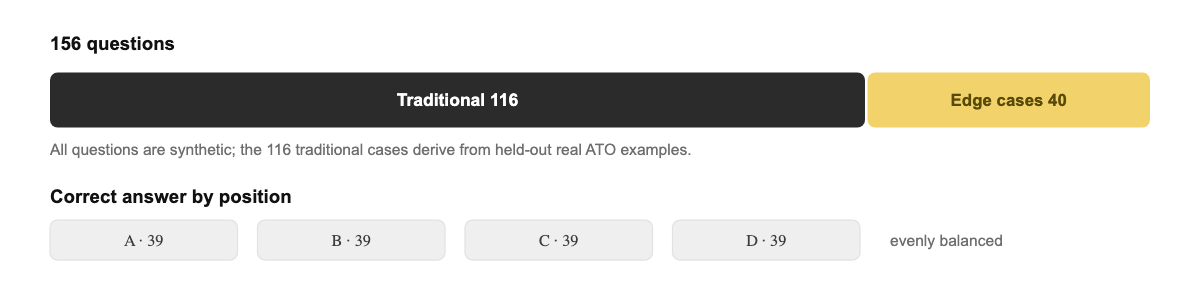
\includegraphics[width=\linewidth]{figures/paper/figure-1.png}
  \caption{\captiontext{The 156 public questions split into 116 traditional calculation cases and 40 edge cases; answer positions are balanced 39 each across A-D.}}
\end{figure}

\section{A CGT example shows the pattern}

The CGT example below shows how the benchmark turns a rule into a bounded task. The model must notice the ownership period, apply the 50\% CGT discount, and choose the resulting capital gain.

\begin{questionbox}
Justin, an Australian resident, buys a block of land. He owns it for 18 months and sells it, making a capital gain before discount of \$10,000. He has no capital losses. What capital gain will Justin declare after applying the CGT discount?

\begin{center}
\begin{tabular}{>{\bfseries}p{0.06\linewidth}p{0.18\linewidth}p{0.62\linewidth}}
A & \$5,000 & Correct: \$10,000 halved by the 50\% discount \\
B & \$10,000 & Forgot to apply the discount \\
C & \$2,500 & Applied the discount twice \\
D & \$20,000 & Inverted the rate (divided by 0.5) \\
\end{tabular}
\end{center}
\end{questionbox}

The correct answer is \$5,000. The other options encode named mistakes: forgetting the discount, applying it twice, or inverting the rate. A wrong answer therefore becomes more than a miss; it becomes a failure signal.

\begin{figure}[htbp]
  \centering
  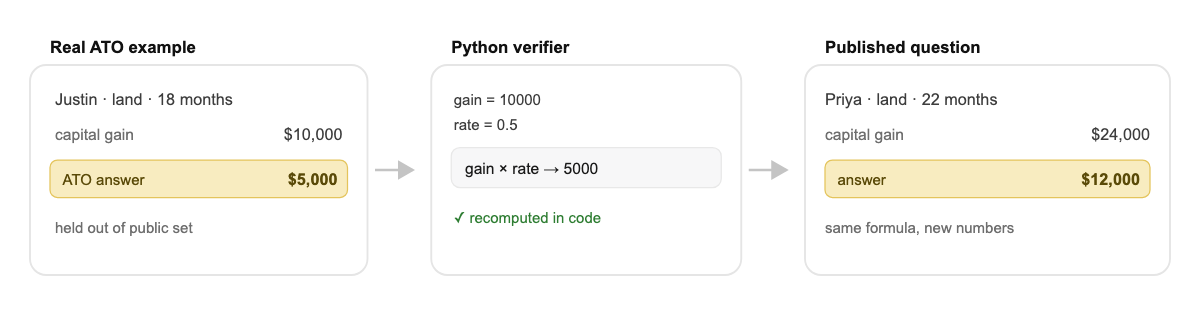
\includegraphics[width=\linewidth]{figures/paper/figure-2.png}
  \caption{\captiontext{A held-out ATO example becomes a formula, the verifier recomputes the result, and the public question uses new numbers.}}
\end{figure}

\section{Traditional and edge cases}

All 156 public questions are synthetic: each uses a new name, new numbers, or both, so the original ATO answer no longer fits. The split has two jobs. Traditional cases test whether the model can perform the standard calculation; edge cases test whether it notices the fact that changes the outcome.

\textbf{Traditional cases:} each of the 116 cases starts from a real ATO worked example. We keep the verified calculation and reword the text, changing only the taxpayer name and numbers (for example, ``Jim'' to ``Jess'', or \$4,500 to \$6,500). The 116 verbatim originals are held out and not published.

Holding out the originals reduces answer recall. ATO worked examples are public and may appear in model training data, so a model could otherwise return the published answer instead of calculating it. New numbers force the calculation, but they do not remove the source entirely: a determined agent might still find the original online.

\textbf{Edge cases:} the 40 edge cases are deliberate traps and boundaries. They test whether a model notices the exception, not just whether it knows the standard case:

\begin{itemize}
  \item \textbf{Single flipped fact:} an asset held just under 12 months, so the CGT discount is denied.
  \item \textbf{Exact threshold:} a value placed directly on a rate, cap, or eligibility boundary.
  \item \textbf{Loss or zero:} a scenario where the result is a loss or nil.
  \item \textbf{Multi-step chain:} a question that needs several steps in sequence.
\end{itemize}

For a trap, one wrong option is the naive answer: the result a model gets if it misses the exception and applies the standard rule.

\begin{figure}[htbp]
  \centering
  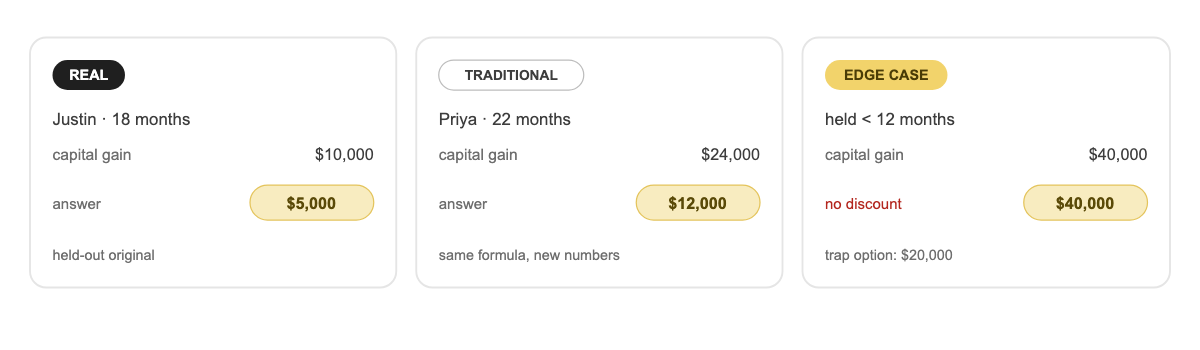
\includegraphics[width=\linewidth]{figures/paper/figure-3.png}
  \caption{\captiontext{One calculation can produce three eval targets: the held-out original, a published traditional case with new numbers, and an edge case that changes the rule.}}
\end{figure}

\section{Answers you can check with code}

Every question ships with a stored formula and named inputs that recompute the correct answer. A small calculator evaluates only arithmetic (\texttt{+ - * / // \% **}) and four functions (\texttt{min}, \texttt{max}, \texttt{round}, \texttt{abs}). This creates three evaluation modes:

\begin{itemize}
  \item \textbf{Grade a submission:} pass a CSV of \texttt{id,answer}; the verifier reports overall and per-topic accuracy.
  \item \textbf{Recompute one case:} point the verifier at a question id to rerun its formula and confirm the key.
  \item \textbf{Expose a calculator:} let the agent call the calculator while it solves, so it computes the number rather than relying on recall.
\end{itemize}

\begin{Verbatim}[fontsize=\small,frame=single,rulecolor=\color{line}]
python verifier.py grade my_answers.csv
python verifier.py verify --id Q001
python verifier.py calc "(880000 - 615000) * 0.5"
\end{Verbatim}

\section{Using the benchmark to evaluate an agent}

The benchmark can run against any conversational or API agent. The simplest workflow is intentionally narrow: present one question, ask for one letter, and grade the answer against the key.

\textbf{Start with one canonical prompt:} show the question and its four options, then ask for one letter.

\begin{Verbatim}[fontsize=\small,frame=single,rulecolor=\color{line}]
Answer this Australian tax question.
Return only A, B, C, or D.

{question}
\end{Verbatim}

Use this prompt for comparable scores. Custom prompts are allowed, but they should be labelled as custom-prompt runs.

From this base, run optional variants:

\begin{itemize}
  \item \textbf{Zero-shot:} use the prompt above, with no reasoning requested.
  \item \textbf{Explanation-first:} ask for a short explanation before the final letter, so reviewers can inspect why the model answered correctly or incorrectly.
  \item \textbf{Conversational framing:} embed the question in a dialogue and optionally ask for a confidence level.
\end{itemize}

\section{Tool-use mode}

Tool access is part of the run setup. Report whether web, tax databases, or calculator tools were allowed.

A calculator is useful either way because it separates two skills: choosing the right tax rule and doing the arithmetic. Retrieval can also be valid to test, but it should be measured as retrieval-assisted performance rather than mixed into a closed-book score.

Prompt text is not a security boundary. If an agent has filesystem tools, it should not be run from a directory containing the answer key. The public runner executes CLI agents from an isolated temporary directory by default, with no \texttt{answer.csv} or \texttt{exam.csv} present.

\section{What to measure}

Overall accuracy is useful, but a good evaluation might also measure:

\begin{itemize}
  \item \textbf{Per-topic accuracy:} group results by tax area. A model may perform well on CGT but poorly on GST, FBT, or Division 7A.
  \item \textbf{Edge-case accuracy:} score the 40 edge cases separately. This shows whether the model handles traps and boundaries, not just standard examples.
  \item \textbf{Robustness:} paraphrase questions or make small wording changes. Accuracy should stay stable if the model understands the underlying rule.
  \item \textbf{Error patterns:} use the labelled wrong options to identify common failure modes: missed thresholds, unavailable discounts, wrong income years, or skipped steps.
\end{itemize}

These measures make the benchmark more useful than a single score. They show where an agent is reliable and where it needs more work.

\section{What this benchmark does not claim}

This benchmark is a test tool, not tax or financial advice.

It is not endorsed by the ATO. All figures should be verified before anyone relies on them in real work.

The benchmark is also tied to income years. Australian tax rates, thresholds, and rules can change. An answer that is correct for one income year may be wrong for another.

Finally, the questions are derived rather than verbatim. The dataset changes names and numbers, and the answer key cites the governing rule rather than relying on the original wording of the ATO example.

\section{Why this matters}

AI tax agents are moving from demos into real workflows.

This benchmark gives builders and evaluators a practical way to measure this: can this agent actually calculate Australian tax, or is it just guessing well?

\end{document}
